% Source: graduate-coursework/Prior_Semesters/Fa25/EMCH501/HW3/HW3.tex
% Description: The undamped spring-mass system.

\documentclass[border=4pt]{standalone}
\usepackage{amsmath}
\usepackage{amssymb}
\usepackage{graphicx}
\usepackage{pgfplots}
\usepackage{tikz}
\usepackage{xcolor}
\pgfplotsset{compat=1.18}
\usetikzlibrary{shapes.geometric, arrows.meta, positioning, decorations.pathmorphing, patterns}

\definecolor{USC_Garnet}{HTML}{73000A}
\definecolor{USC_Sandstorm}{HTML}{FFF2E3}
\definecolor{USC_Black90}{HTML}{565656}
\definecolor{USC_Black10}{HTML}{ECECEC}
\definecolor{USC_Honeycomb}{HTML}{65780B}

\begin{document}
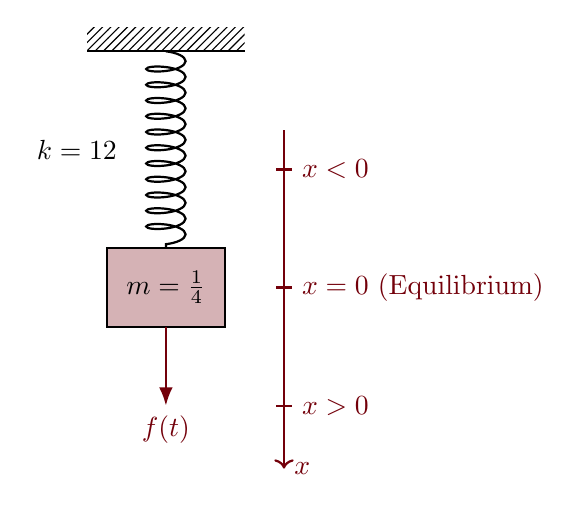
\begin{tikzpicture}[scale=1]
        
        % --- 1. Physical System Diagram (Left Side) ---
        
        % Support/Ceiling
        \fill[pattern=north east lines] (-1, 0) rectangle (1, 0.3);
        \draw[thick] (-1, 0) -- (1, 0);
        
        % Spring (Resting/Equilibrium position roughly)
        \draw[decoration={aspect=0.3, segment length=2mm, amplitude=2.5mm, coil}, decorate, thick] (0,0) -- (0,-2.5);
        
        % Mass
        \draw[fill= USC_Garnet!30, thick] (-0.75, -2.5) rectangle (0.75, -3.5);
        \node at (0, -3) {$m=\frac{1}{4}$};
        
        % Coordinate System (x-axis pointing down)
        \draw[->, thick, USC_Garnet] (1.5, -1) -- (1.5, -5.3) node[right] {$x$};
        \draw[thick, USC_Garnet] (1.4, -3.0) -- (1.6, -3.0) node[right] {$x=0$ (Equilibrium)};
        \draw[thick, USC_Garnet] (1.4, -1.5) -- (1.6, -1.5) node[right] {$x < 0$};
        \draw[thick, USC_Garnet] (1.4, -4.5) -- (1.6, -4.5) node[right] {$x > 0$};

        % Force Vector
        \draw[-Latex, USC_Garnet, thick] (0, -3.5) -- (0, -4.5) node[below] {$f(t)$};

        % Labels
        \node[anchor=east] at (-0.5, -1.25) {$k=12$};


    \end{tikzpicture}
\end{document}
